\section{Introduction}

\Xten{}~\cite{X10} is an experimental new language currently under development at
IBM in collaboration with academic partners. The \Xten{} effort is part of
the IBM PERCS project (Productive Easy-to-use Reliable Computer Systems)
in the DARPA program on High Productivity Computer Systems. The PERCS
project is focused on a hardware-software co-design methodology to
integrate advances in chip technology, architecture, operating systems,
compilers, programming language and programming tools to deliver new
adaptable, scalable systems that will provide an order-of-magnitude
improvement in development productivity for parallel applications. It is
expected that applications written in \Xten{} will execute over
high-performance interconnects using low-level communication libraries.
\Xtenlib{} is a library that is built on top of low level communication
libraries, like LAPI~\cite{LAPI} and provides a runtime target API for
the \Xten{} compiler.

\begin{figure}
\center
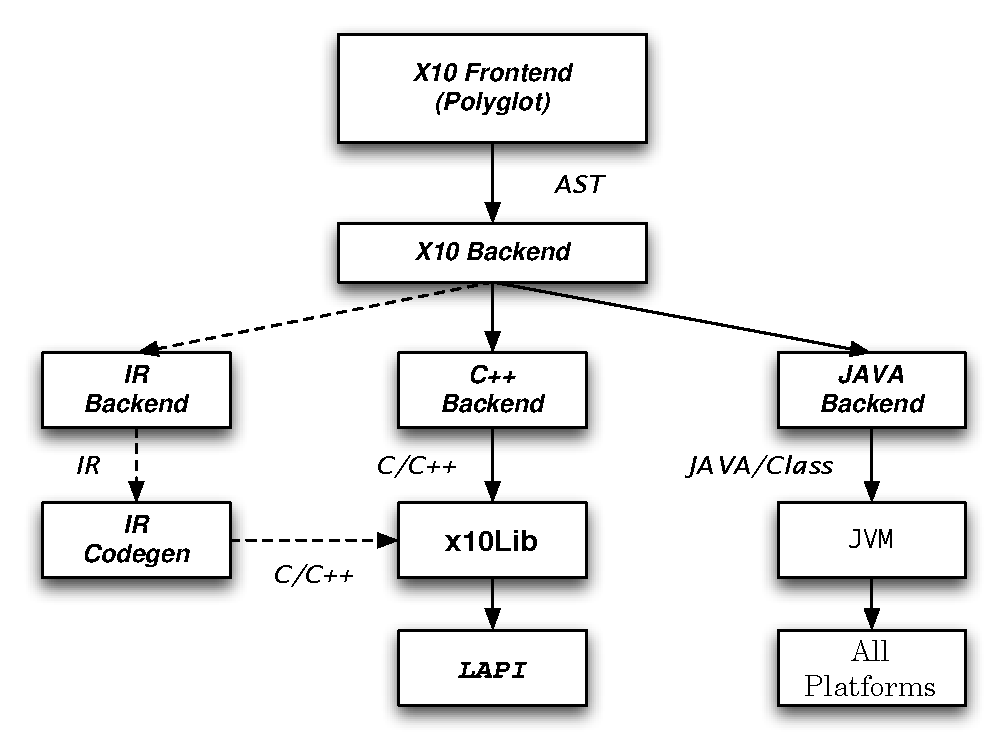
\includegraphics[scale=0.5]{figs/x10-block.pdf}
\caption{Overview of Implementation Strategies for \Xten{}}
\label{fig:x10-block}
\end{figure}

Figure~\ref{fig:x10-block} depicts the implementation strategy for the
\Xten{} programming language. The \Xten{} backend is responsible for
converting \Xten{} programs to map to either the C++ backend or the
{\sc{Java}} backend. The C++ backend then links with the \Xtenlib{} API
to run over high-performance interconnects on multiple places, i.e. on
multiple processes spread out over different nodes connected by a
network. The {\sc{Java}} backend is used to run \Xten{} programs in the
context of a JVM. In this document, we will focus only on \Xtenlib{}.
The Low-Level Communication API (LAPI)~\cite{LAPI} is utilized by
\Xtenlib{} to communicate over the network. This provides a highly
optimized runtime library.

The primary purpose of \Xtenlib{} is to provide the \textit{Partitioned
Global Address Space (PGAS)} required by \Xten{} along with methods to
deploy and execute \Xten{} programs. \Xtenlib{} provies the PGAS by
logically dividing up the address space among the various computing
processes and managing the book-keeping required to convert
pointer-dereferences into communication calls. \Xtenlib{} borrows the
process management framework from Parallel Operating Environment (POE),
which is ordinarily used to run MPI applications. Thus, inheriting a
highly optimized and scalable runtime environment.

The rest of this Section outlines the design goals and summarizes
desired functionality.

\subsection{Design Goals}

We list the following explicit design goals for \Xtenlib:

\begin{itemize}

	\item The design should efficiently execute programs that are
		communication-intensive and programs that are
		compute-intensive. It should permit the user to specify
		how many processes to run on each node of the cluster,
		how many places to run on each process, and how many
		threads to assign to each place.

	\item \Xtenlib{} should permit current C/C++ MPI programmers to
		program with \Xten{} concepts such as global shared memory,
		multi-threaded places, asyncs, futures, clocks and one-sided memory
		operations.

	\item \Xtenlib{} should export an interface to the compiler
		similar in spirit to the interface provided by the Java Virtual
		Machine. The interface must provide specialized entry points for
		common cases (e.g.{} allocating 1D, 2D, 3D Rectangular arrays).

	\item It should be possible to spawn activities in the current 
		process or on remote processes, and detect quiescence and
		termination of these activities.

	\item The library should be efficiently implementable on top of
		LAPI~\cite{LAPI} and ARMCI~\cite{ARMCI} and other similar
		high-peformance messaging systems.

\end{itemize}

Initially bindings will be provided for C and C++. Bindings for Fortran
and Java are also planned.

The following are explicitly {\em not} design goals for \Xtenlib:

\begin{itemize}
	\item \Xtenlib{} is a C/C++ API: it will not offer any explicit
		support for statically proving properties such as deadlock-freedom.
		(Such properties are provided at the language level for \Xten).

	\item This version of \Xtenlib{} will not provide any support for
		garbage collection. The user is responsible for automatically managing
		the lifetime of objects.

	\item This version of \Xtenlib{} will not support the dynamic creation of places.

	\item This version of \Xtenlib{} will not support checkpointing of
		places. It will not support migration of places from one process to
		another.

	\item This version of \Xtenlib{} will not support distributed
		data strutures other than arrays.
\end{itemize}

\subsection{Summary of desired functionality}

\Xtenlib{} provides functions to do the following:

\begin{itemize}
	\item Get a remote (globally valid) reference for a local data structure.
		Such references can be passed from place to place and still remain
		valid. Two such references may be checked locally (without any
		communication) to determine if they point to the same data
		structure.

	\item Spawn an async at a specified place, with a given function pointer
		and arguments, and clocked on given clock set. (The place may be
		specified either through a specific structure naming the place or
		through a remote reference.)

	\item Create a clock, and perform clock operations (next, resume, drop).

	\item Spawn a future at a given place, with a given function
		pointer and arguments, and clocked on given clock set, and return
		the future.

	\item Force the future. (This causes the current thread to block until the
		future value has been computed, and must therefore be performed at
		the top-level.)

	\item Spawn activities in parallel at a given vector of places.

	\item Terminate the current activity. (This does not terminate the current
		pthread, merely causes it to look for another activity to execute.)

	\item Call finish to suspend on the termination of all asynchronous
		activities in the scope of the finish.

	\item Perform an atomic operation with a given piece of code.
	\item Throw an exception (to be caught by an enclosing finish).

	\item Initialize a global data structure by allocating local arrays at
		given places.

	\item Perform operations on the local portion of an array --
		read/write/atomically update/iterate over elements in storage
		order/region order.

	\item Copy a portion of an array from the local place to a remote
		place, or from a remote place into the local place.

	\item Perform reduction operations on a global array.

	\item Free global or local data structure.
\end{itemize}

Additional intrinsics capturing common idioms for communication that
can be efficiently executed on modern hardware will also be provided.

\paragraph{Target architecture}
The intended target architecture for the initial \Xtenlib{}
implementation is a cluster of SMPs connected through a high
performance switch. For instance, a cluster of 64-way Power5 SMPs
connected by a Federation switch. We view this as the best current
approximation to the PERCS machine being designed for 2010. We expect
the current design to be applicable to the PERCS machine though the
details may change significantly.
